\chapter{跑步} \label{chap:chap3}

如果你能用六十秒的长跑来填补这无情的一分钟……
\begin{flushright}
	——拉迪亚德$\cdot$吉卜林
\end{flushright}


\begin{figure}[!htb]
	\centering
	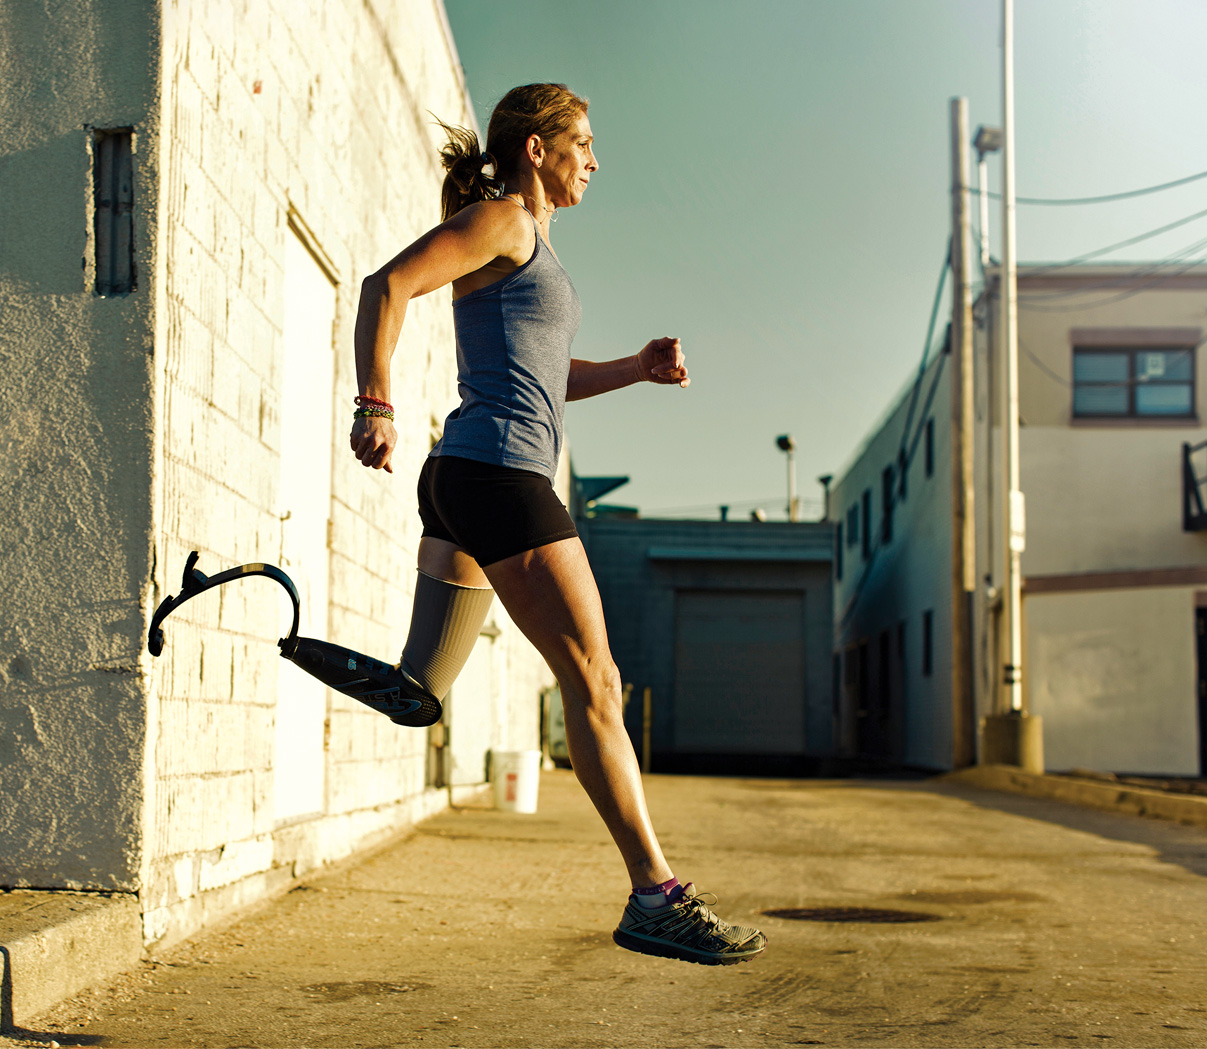
\includegraphics[width=1.0\linewidth]{chap3/3_0}
	% 加星号(*)表示不加编号
	\caption*{ \label{fig:3_0}}
\end{figure}

看过《侏罗纪公园》的人可能都记得那个标志性的场景:
一辆吉普车试图超越一只追赶的霸王龙。
有趣的是,这个场景与电影上映时(1993年)古生物学家的普遍看法相符。
当时人们认为霸王龙的奔跑速度可以达到 40 公里/小时,一些科学家甚至认为它的速度甚至可能更快。
以这样的速度,它在土路上完全可以超过一辆吉普车。


然而,自 2002 年约翰$\cdot$哈钦森(John Hutchinson)开创性论文以来,近期的生物力学研究表明,霸王龙可能根本无法奔跑。
即使它能跑,也可能无法达到 40 公里/小时的速度。
哈钦森通过模拟霸王龙,证明要达到这样的速度,其 86\% 的体重必须由腿部肌肉构成,留给其庞大的尾巴、头部和躯干的空间非常有限。
为了产生足够大的地面反作用力,它需要将如此大的质量分配给腿部肌肉,而这种反作用力在奔跑时通常超过体重的两倍。


对恐龙、大象和袋鼠等动物的研究有助于我们理清对人类跑步的理解:
是什么驱动着从步行到跑步的转变,又是什么限制了跑步速度。
地面反作用力的测量揭示了为什么跑步时比步行时更容易受伤,以及如何设计跑道来降低受伤率并提高速度。


在本章中,我们将使用简单的力学模型来探讨这些问题。
这些模型包含弹簧,用于表示肌肉和肌腱的弹性特性,并揭示弹性能量的储存和释放如何提高跑步效率。
首先,我们定义跑步步态周期,并研究其中涉及的力和弹性机制。
然后,我们将探索一些原理,帮助你设计跑道、跑鞋和假肢,从而实现快速高效的跑步。
我们还会研究从步行过渡到跑步时步态和能量消耗的变化。


\section{跑步步态周期}

跑步步态周期由单腿支撑和腾空交替的阶段组成(图~\ref{fig:3_1})。
与步行类似,一个跑步步态周期由同一条腿连续 2 次触地事件定义,其中对侧腿的触地发生在半程。
每条腿都有一个\textit{支撑期}(脚与地面接触)和一个\textit{摆动期}(脚离地)。
支撑期始于脚触地,结束于脚趾离地,在人类跑步过程中约占步态周期的 30\% 到 45\%,但在高速冲刺过程中可能只占 25\% 或更少。
回想一下,步行时支撑期的持续时间会随着步行速度的增加而缩短。
因此,随着步行速度的增加,双腿支撑的持续时间会缩短。
如果进一步提高速度,每条腿对应的支撑期最终将持续不到步态周期的一半,从而进入腾空期。


\begin{figure}[!htb]
	\centering
	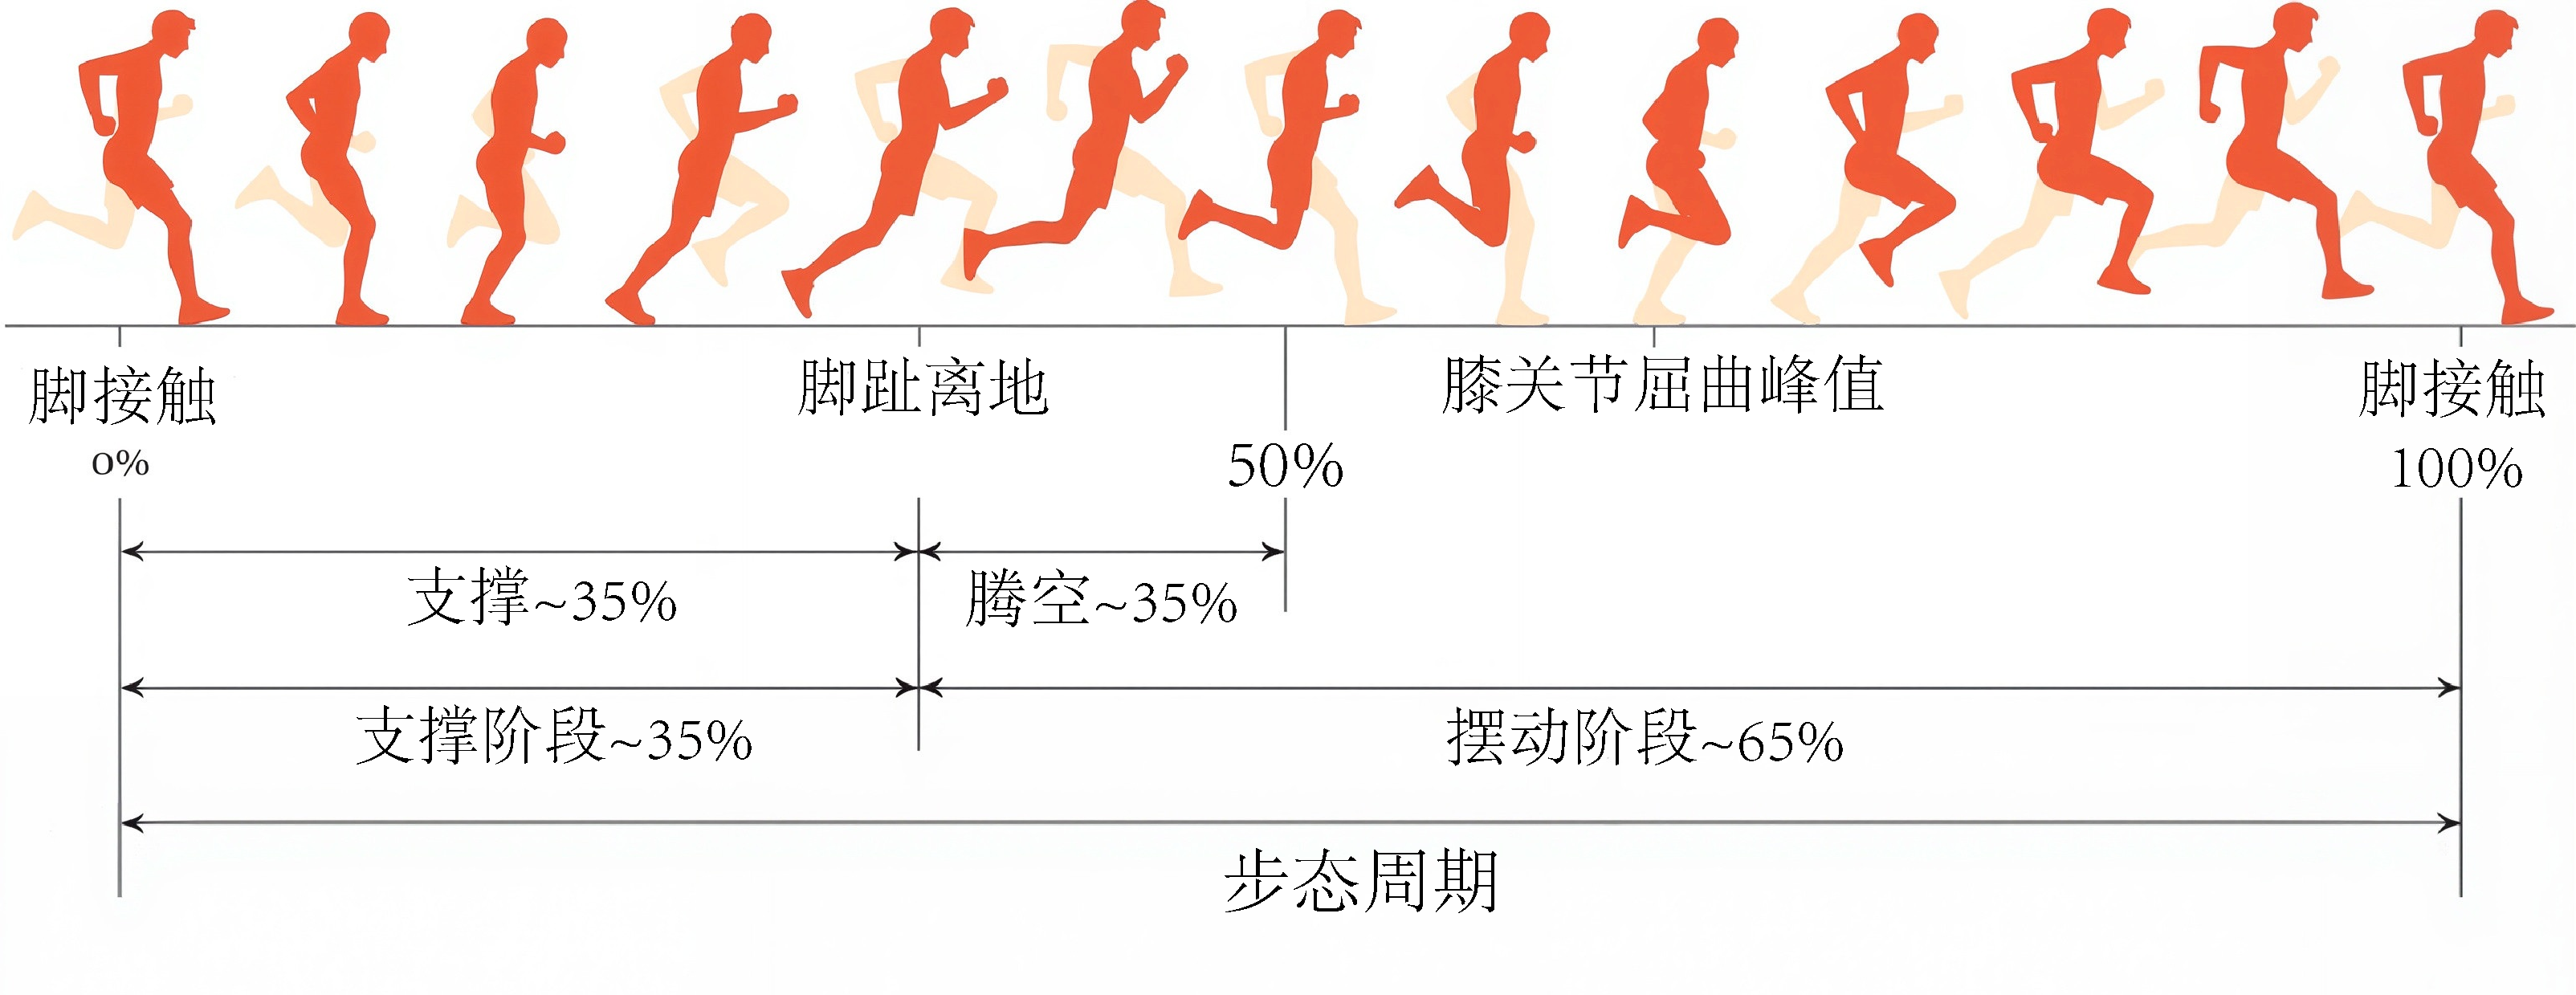
\includegraphics[width=1.0\linewidth]{chap3/3_1}
	\caption{跑步步态周期及其组成事件(例如,脚部触地)和阶段(例如,支撑)。
		站立和摆动的时间百分比会随着跑步速度和风格而变化。 \label{fig:3_1}}
\end{figure}

腾空阶段的存在是我们区分行走和跑步的一个方式。
事实上,人们很容易相信它是跑步的特征,不仅对人类如此,对其他动物也是如此。
然而,我们很快就会看到,当我们从行走步态转换为跑步步态时,会发生另一种质的变化,从生物力学的角度来看,这一点更为重要。


用于量化跑步步态周期的指标与用于步行的指标类似。
步长是两个连续足迹之间沿行进线的距离。
连续两步所走的距离,或一个步态周期所走过的距离,称为步长。
足部接触事件发生的速率(相当于步长持续时间的倒数)称为步频;
迈步的速率称为步频。
跑步速度可以用步长与步频的乘积来计算,
或者,也可以用步长与步频的乘积来计算:

\begin{equation}
	\text{速度(米/秒)} = \text{步长(米/步)} \times \text{节律(步/秒)} \label{eq:3_1}
\end{equation}

中等跑步速度为 4 米/秒。
在此速度下,支撑期约占步态周期的 35\% 至 40\%,典型的步频为 180 步/分钟,典型的步长约为 1.3 至 1.4 米:

\begin{equation}
	\text{步长} = \frac{4.0 \text{米}}{1 \text{秒}}
				 \times \frac{60 \text{秒}}{1 \text{分钟}}
				 \times \frac{1 \text{分钟}}{180 \text{步}}
				 = 1.33 \text{米/秒}
				 \label{eq:3_2}
\end{equation}

当然,这些数量会随着腿长、跑步风格、鞋类和其他因素而变化。


\section{地面反作用力}

正如我们在第~\ref{chap:chap2}~章中所看到的,我们可以通过测量地面反作用力随时间的变化来深入了解步态的动力学和能量学。
跑步时,地面反作用力的垂直分量在足部触地后迅速上升,并在步态周期的约15\%到20\%处达到最大值(图~\ref{fig:3_2})。
在中等速度跑步时,垂直地面反作用力在约 2 倍体重时达到峰值。
水平地面反作用力在站立的前半段指向后方,使重心减速,之后指向前方。

\begin{figure}[!htb]
	\centering
	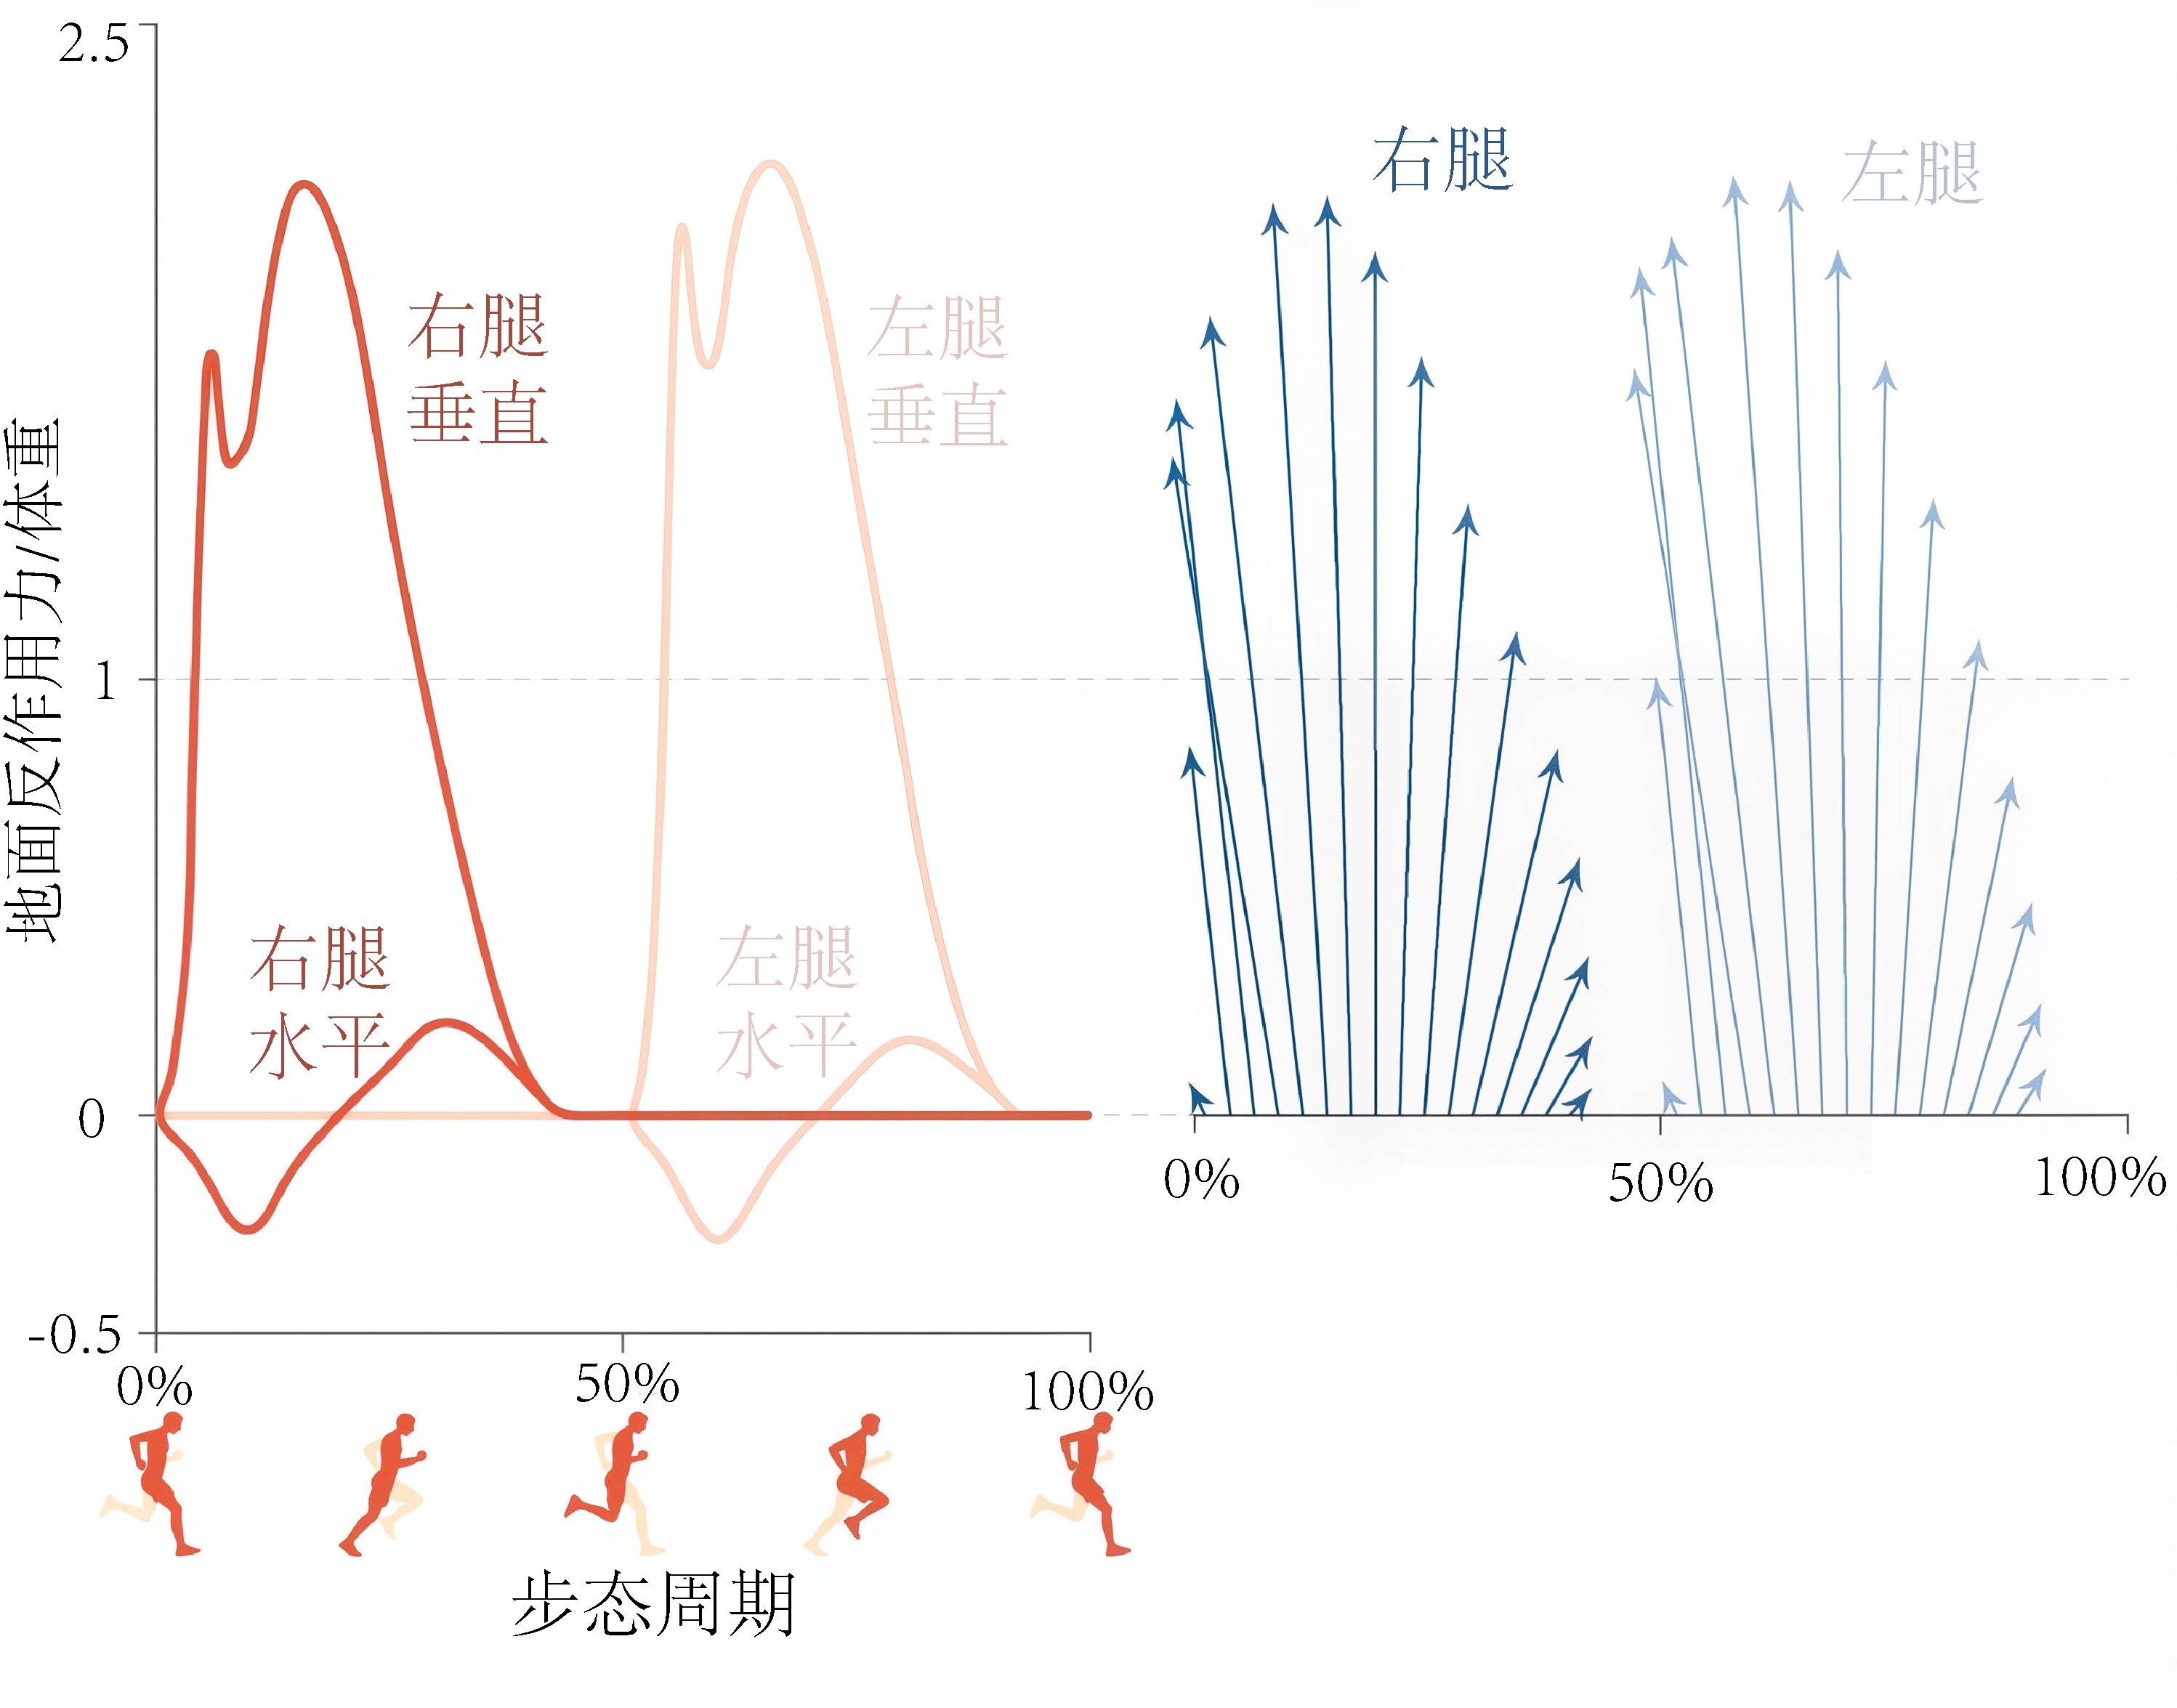
\includegraphics[width=1.0\linewidth]{chap3/3_2}
	\caption{跑步时足跟着地时代表性的地面反作用力。
		图中显示了步态周期内的垂直和水平(前后)分量(左)以及总矢量示意图(右)。
		垂直地面反作用力在足跟着地时出现一个急剧的峰值\cite{yong2020foot}。 \label{fig:3_2}}
\end{figure}

图~\ref{fig:3_2}~显示了后脚掌着地的跑步者(即用脚跟着地的跑步者)身上特有的双峰垂直地面反作用力。
虽然行走时的地面反作用力也有两个峰值,但跑步时第一个峰值较短,是由于脚跟着地产生的。
某些跑步者,尤其是那些从小就赤脚跑步的跑步者,会用前脚掌着地。
对于这些跑步者来说,垂直地面反作用力上升得更平缓,并且只有一个峰值(图~\ref{fig:3_3})。
有人认为这种跑步方式更“自然”,可以防止与冲击相关的伤害,但后续研究对这一结论提出了质疑。
从小就用后脚掌着地的跑步者如果改为用前脚掌着地,尤其是在没有经过适当训练的情况下,可能会有受伤的风险。

\begin{figure}[!htb]
	\centering
	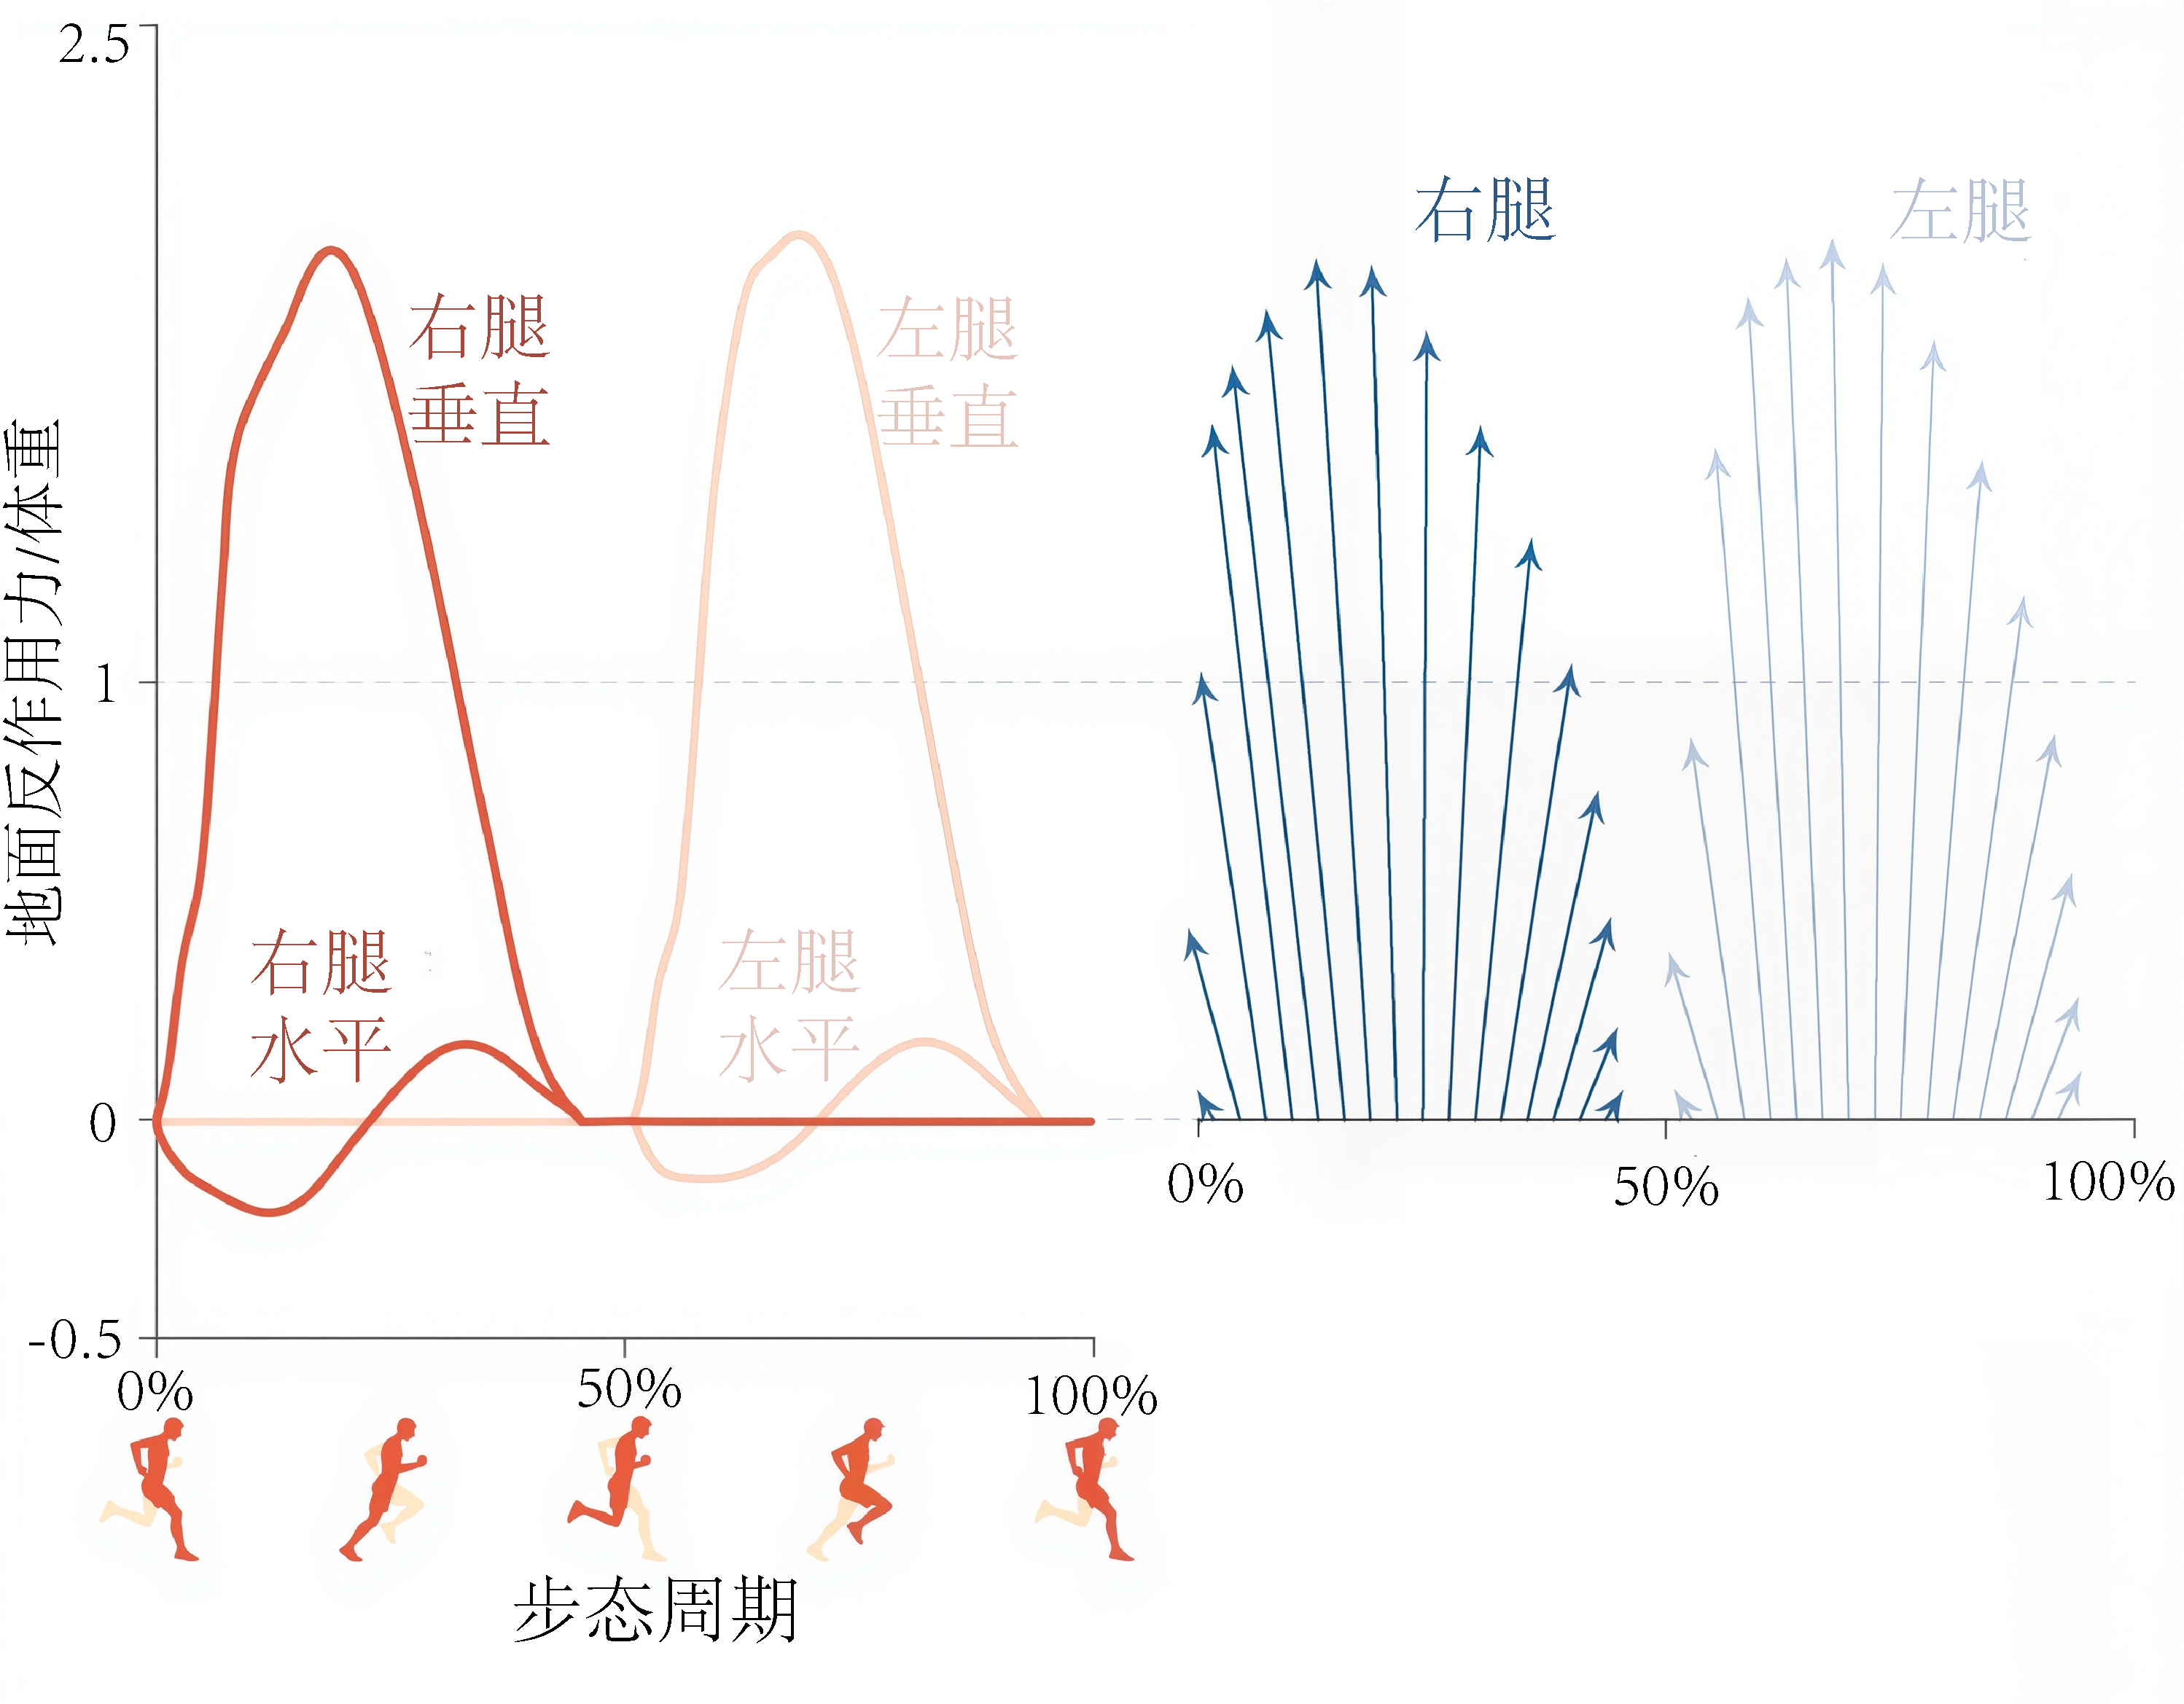
\includegraphics[width=1.0\linewidth]{chap3/3_3}
	\caption{前脚掌落地时,跑步过程中地面反作用力的代表性数据,与图~\ref{fig:3_2}~中的受试者相同。
		垂直地面反作用力没有后脚掌落地时出现的尖峰,这可能有助于降低受伤风险\cite{yong2020foot}。 \label{fig:3_3}}
\end{figure}


跑步时,前向动能和重力势能可以用公式~\ref{eq:2_3}~和公式~\ref{eq:2_4}~计算(图~\ref{fig:3_4})。
在跑步的腾空阶段(忽略空气阻力),前向速度和前向动能最大,且近似恒定。
重心在腾空过程中也最高,因此重力势能也最高。
因此,与行走不同,前向动能和重力势能大约同时达到最大值。
同样,前向动能和重力势能都在站立中期达到最小值,也就是说,当重心最低时,前向速度大约最小。

\begin{figure}[!htb]
	\centering
	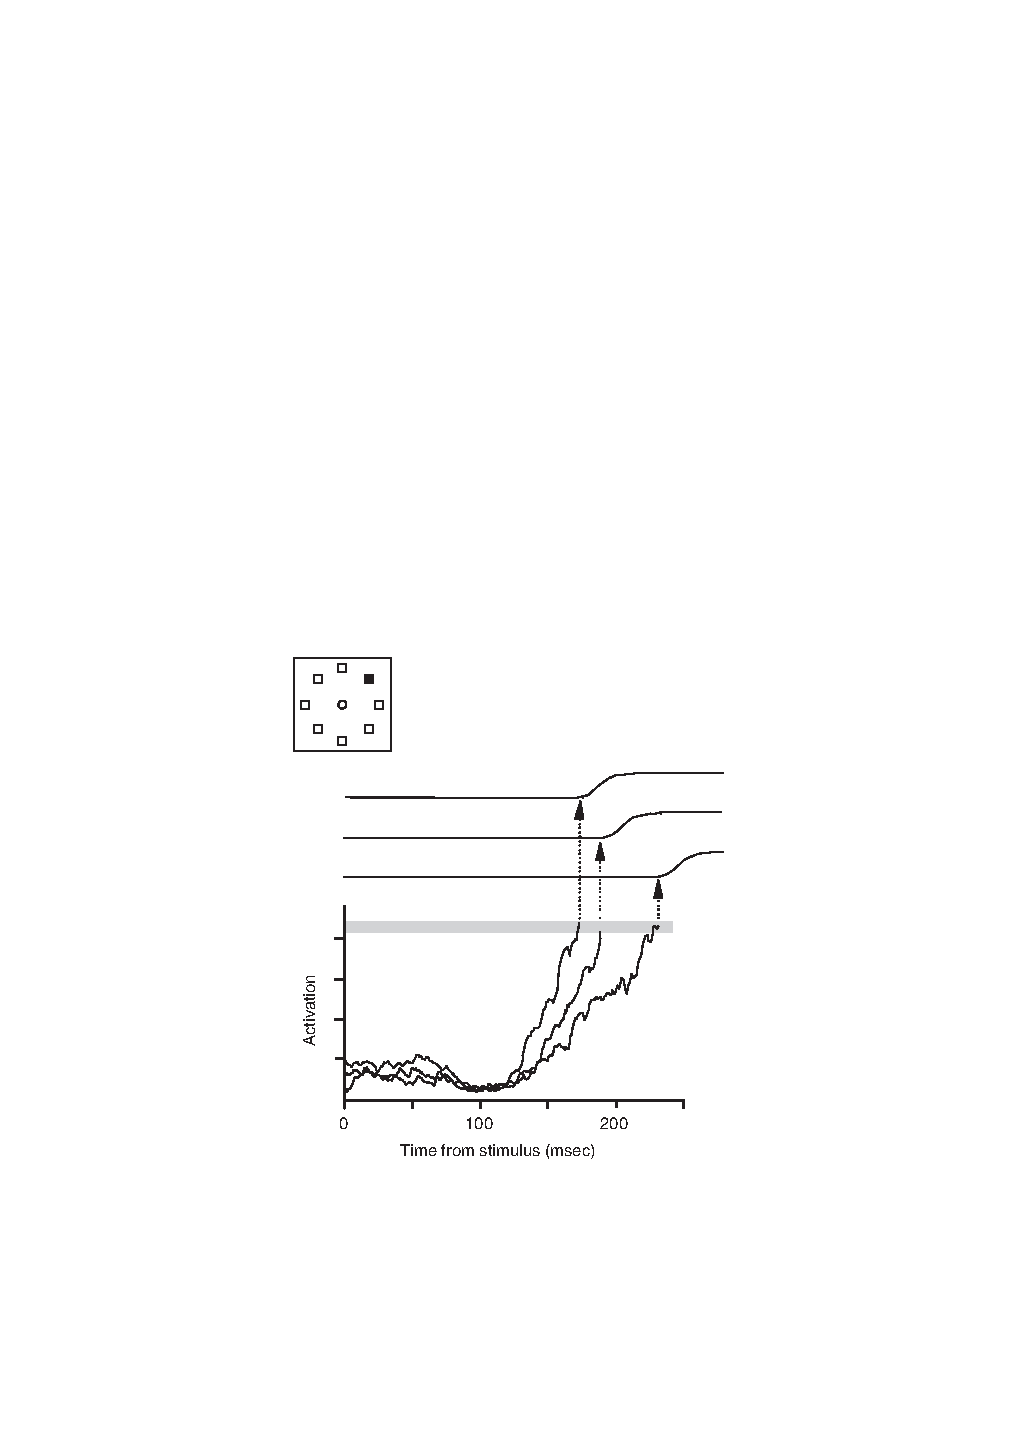
\includegraphics[width=1.0\linewidth]{chap3/3_4}
	\caption{奔跑过程中的代表性重力势能和前向动能。
		飞行过程中,前向动能保持不变\cite{yong2014differences}。 \label{fig:3_4}}
\end{figure}


我们想强调步行和跑步之间的一个根本区别:
在跑步时,我们并非从向前的动能和重力势能的交换中获益,而是在肌肉和肌腱的伸展和回弹过程中储存和释放弹性势能。
这一观察结果暗示了一种如图~\ref{fig:3_5}~所示的跑步模型。
在该模型中,质量在站立中期达到最低点,此时质心的向前速度也最小,这与我们在实验数据中发现的情况相似。
我们腿部如同弹簧般的运动使跑步成为一种能量高效的步态。

\begin{figure}[!htb]
	\centering
	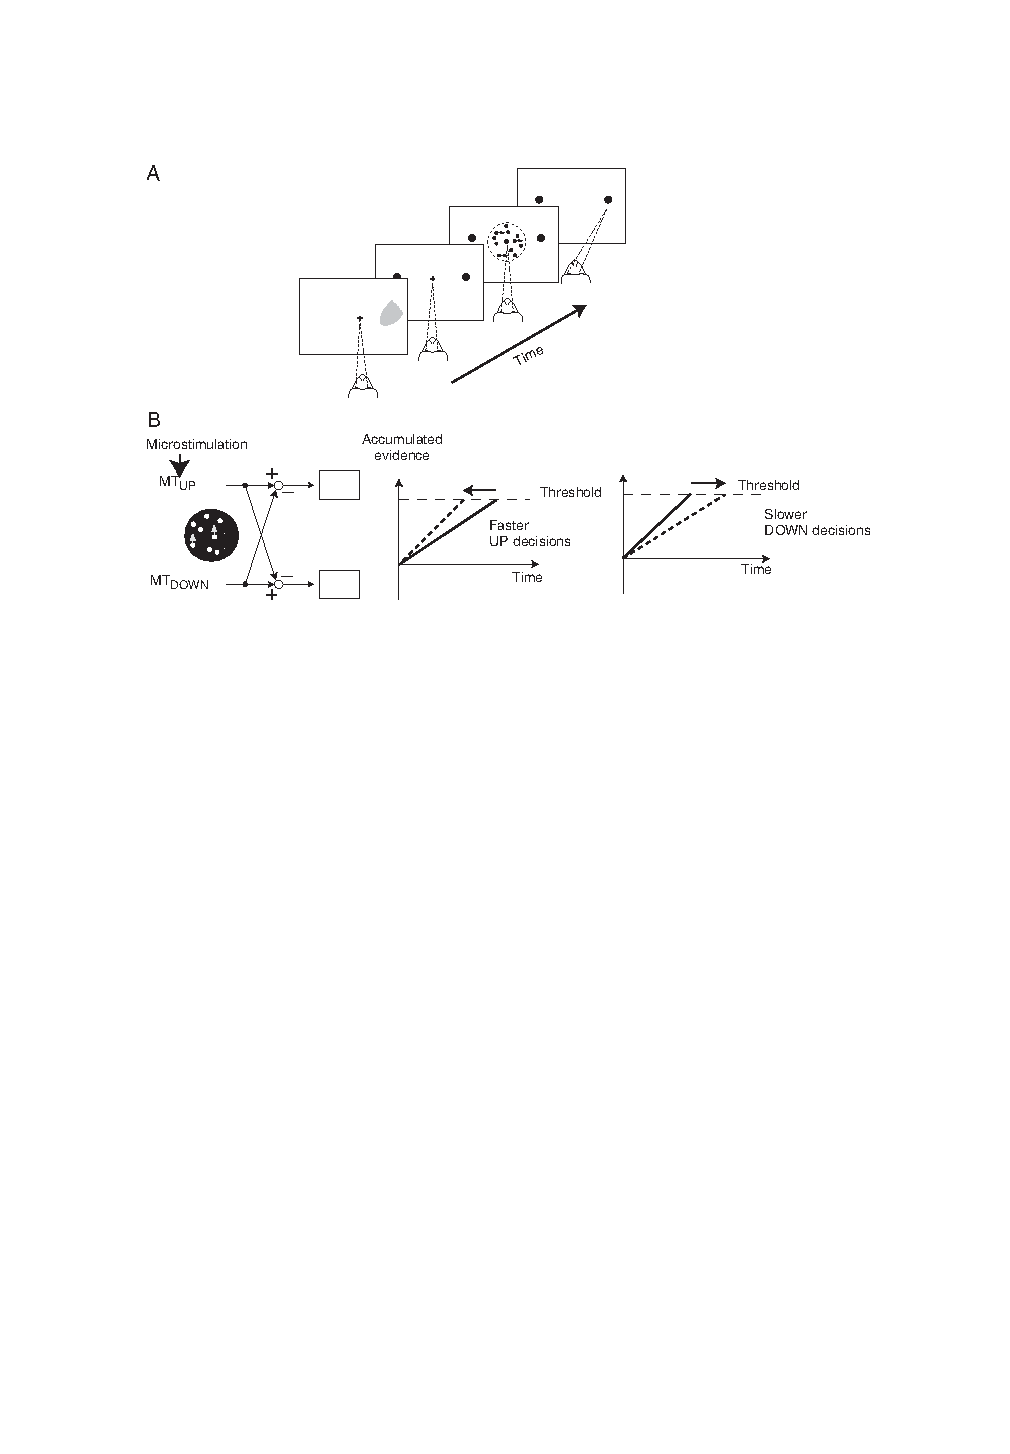
\includegraphics[width=1.0\linewidth]{chap3/3_5}
	\caption{跑步的站立阶段(左)及其质量弹簧模型(右)。
		在该模型中,身体的质量被集中到一个点质量上,该点质量位于代表腿部的无质量线性弹簧的顶部。
		弹簧压缩,质量在站立中期达到最低点,此时质量的前进速度也最低。 \label{fig:3_5}}
\end{figure}


正如我们在第~\ref{chap:chap2}~章中看到的,大象即使在尽可能快地移动时也没有飞行阶段。
因此,你可能会认为大象不会跑。
但事实上,它们似乎有一种“格劳乔式行走”,膝盖弯曲,重力势能和向前动能的波动同步。
从生物力学的角度来看,这种同步意味着大象在某种意义上是在奔跑。
就像人类一样,这些厚皮动物利用腿作为弹簧来储存能量,如图~\ref{fig:3_5}~所示。
大象很可能进化出这种不腾空而起的“奔跑”方式,以适应它们巨大的体型。
正如我们将在本书后面看到的,肌肉力量与肌肉的横截面积(长度的平方)成正比,而体重与体积(长度的立方)成正比。
因此,体型巨大的动物与体型较小的动物相比,体型较大的动物具有较低的力量重量比。
这个原理解释了为什么像松鼠这样的小动物可以产生很大的地面反作用力并跳跃几个身长的距离,而大象和霸王龙(它们的大小大致相同)却无法产生足以让它们瞬间飞翔的地面反作用力。



\section{跳跃和跑步中的弹性机制}

另一种能够让我们了解跑步过程中弹性能量储存的动物是袋鼠。
袋鼠的奔跑并非传统意义上的奔跑;
我们通常将它们的动作描述为跳跃。
然而,从生物力学的角度来看,它们使用的机制与人类跑步时类似。


20世纪70年代初,特伦斯$\cdot$道森和理查德$\cdot$泰勒训练袋鼠佩戴面罩,在跑步机上以1至22公里/小时的速度跳跃——这项实验无疑需要高超的动物操控技巧。
面罩让研究人员能够测量动物的代谢能量消耗,而这正是泰勒当时研究的主题。
他针对袋鼠和其他​​动物进行的大量实验,让生物学家们注意到能量消耗是影响动物行为的关键因素。


道森和泰勒发现,低速时,袋鼠不会跳跃,而是采用五足步态,即用尾巴作为与地面的第五个接触点(图~\ref{fig:3_6})。
这种运动方式看起来很笨拙,而且能量效率低下。
事实上,他们发现,当袋鼠以更高的速度(从 1 到 6 公里/小时;图~\ref{fig:3_7}A)蹒跚向前时,能量消耗急剧增加。
五足步态下速度的提升主要通过增加步频实现(图~\ref{fig:3_7}D)。
当速度达到约 6-7 公里/小时时,袋鼠会过渡到跳跃。
图~\ref{fig:3_7}A~中一个引人注目的特征是,当袋鼠的速度超过 7 公里/小时时,运送成本略有下降。
如图~\ref{fig:3_7}C~和 D 所示,在跳跃阶段,它们主要通过增加步幅来提高速度。
步频几乎保持不变。这一结果与袋鼠的质量弹簧模型(类似于图~\ref{fig:3_5})一致,因为弹簧质量的固有频率不会随着其运动幅度的变化而变化。
Dawson和Taylor指出,袋鼠的跟腱非常适合储存和释放弹性能量,并认为这种机制使跳跃更加高效,并使其能够高速跳跃。


大约在这个时候,泰勒在意大利乔瓦尼$\cdot$卡瓦尼亚的实验室里了解到了测力板,于是他带着他的动物(袋鼠、猴子、狗和火鸡)来到米兰,在卡瓦尼亚当时刚刚发明的实验中试用它们。
最终的研究成果发表于1977年,进一步证明了袋鼠会储存弹性能,并在跳跃过程中释放。
在高达30公里/小时的速度下,氧气消耗约占袋鼠加速重心所需能量的三分之一;
剩余的能量必定是由肌肉和肌腱中的弹性储存提供的。


\begin{figure}[!htb]
	\centering
	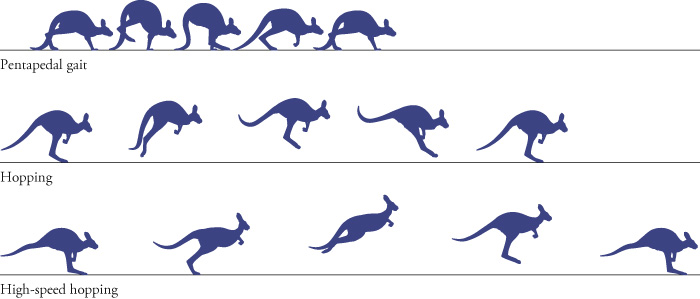
\includegraphics[width=1.0\linewidth]{chap3/3_6}
	\caption{袋鼠的运动方式。
		在慢速运动时,袋鼠采用五足步态(上图),利用尾巴支撑后肢向前移动。
		在高速运动时,袋鼠采用跳跃步态(中图),利用尾巴保持平衡并控制身体倾斜。
		在高速跳跃时(下图),袋鼠的速度可以超过 50 公里/小时\cite{dawson1977kangaroos}。 \label{fig:3_6}}
\end{figure}


\begin{figure}[!htb]
	\centering
	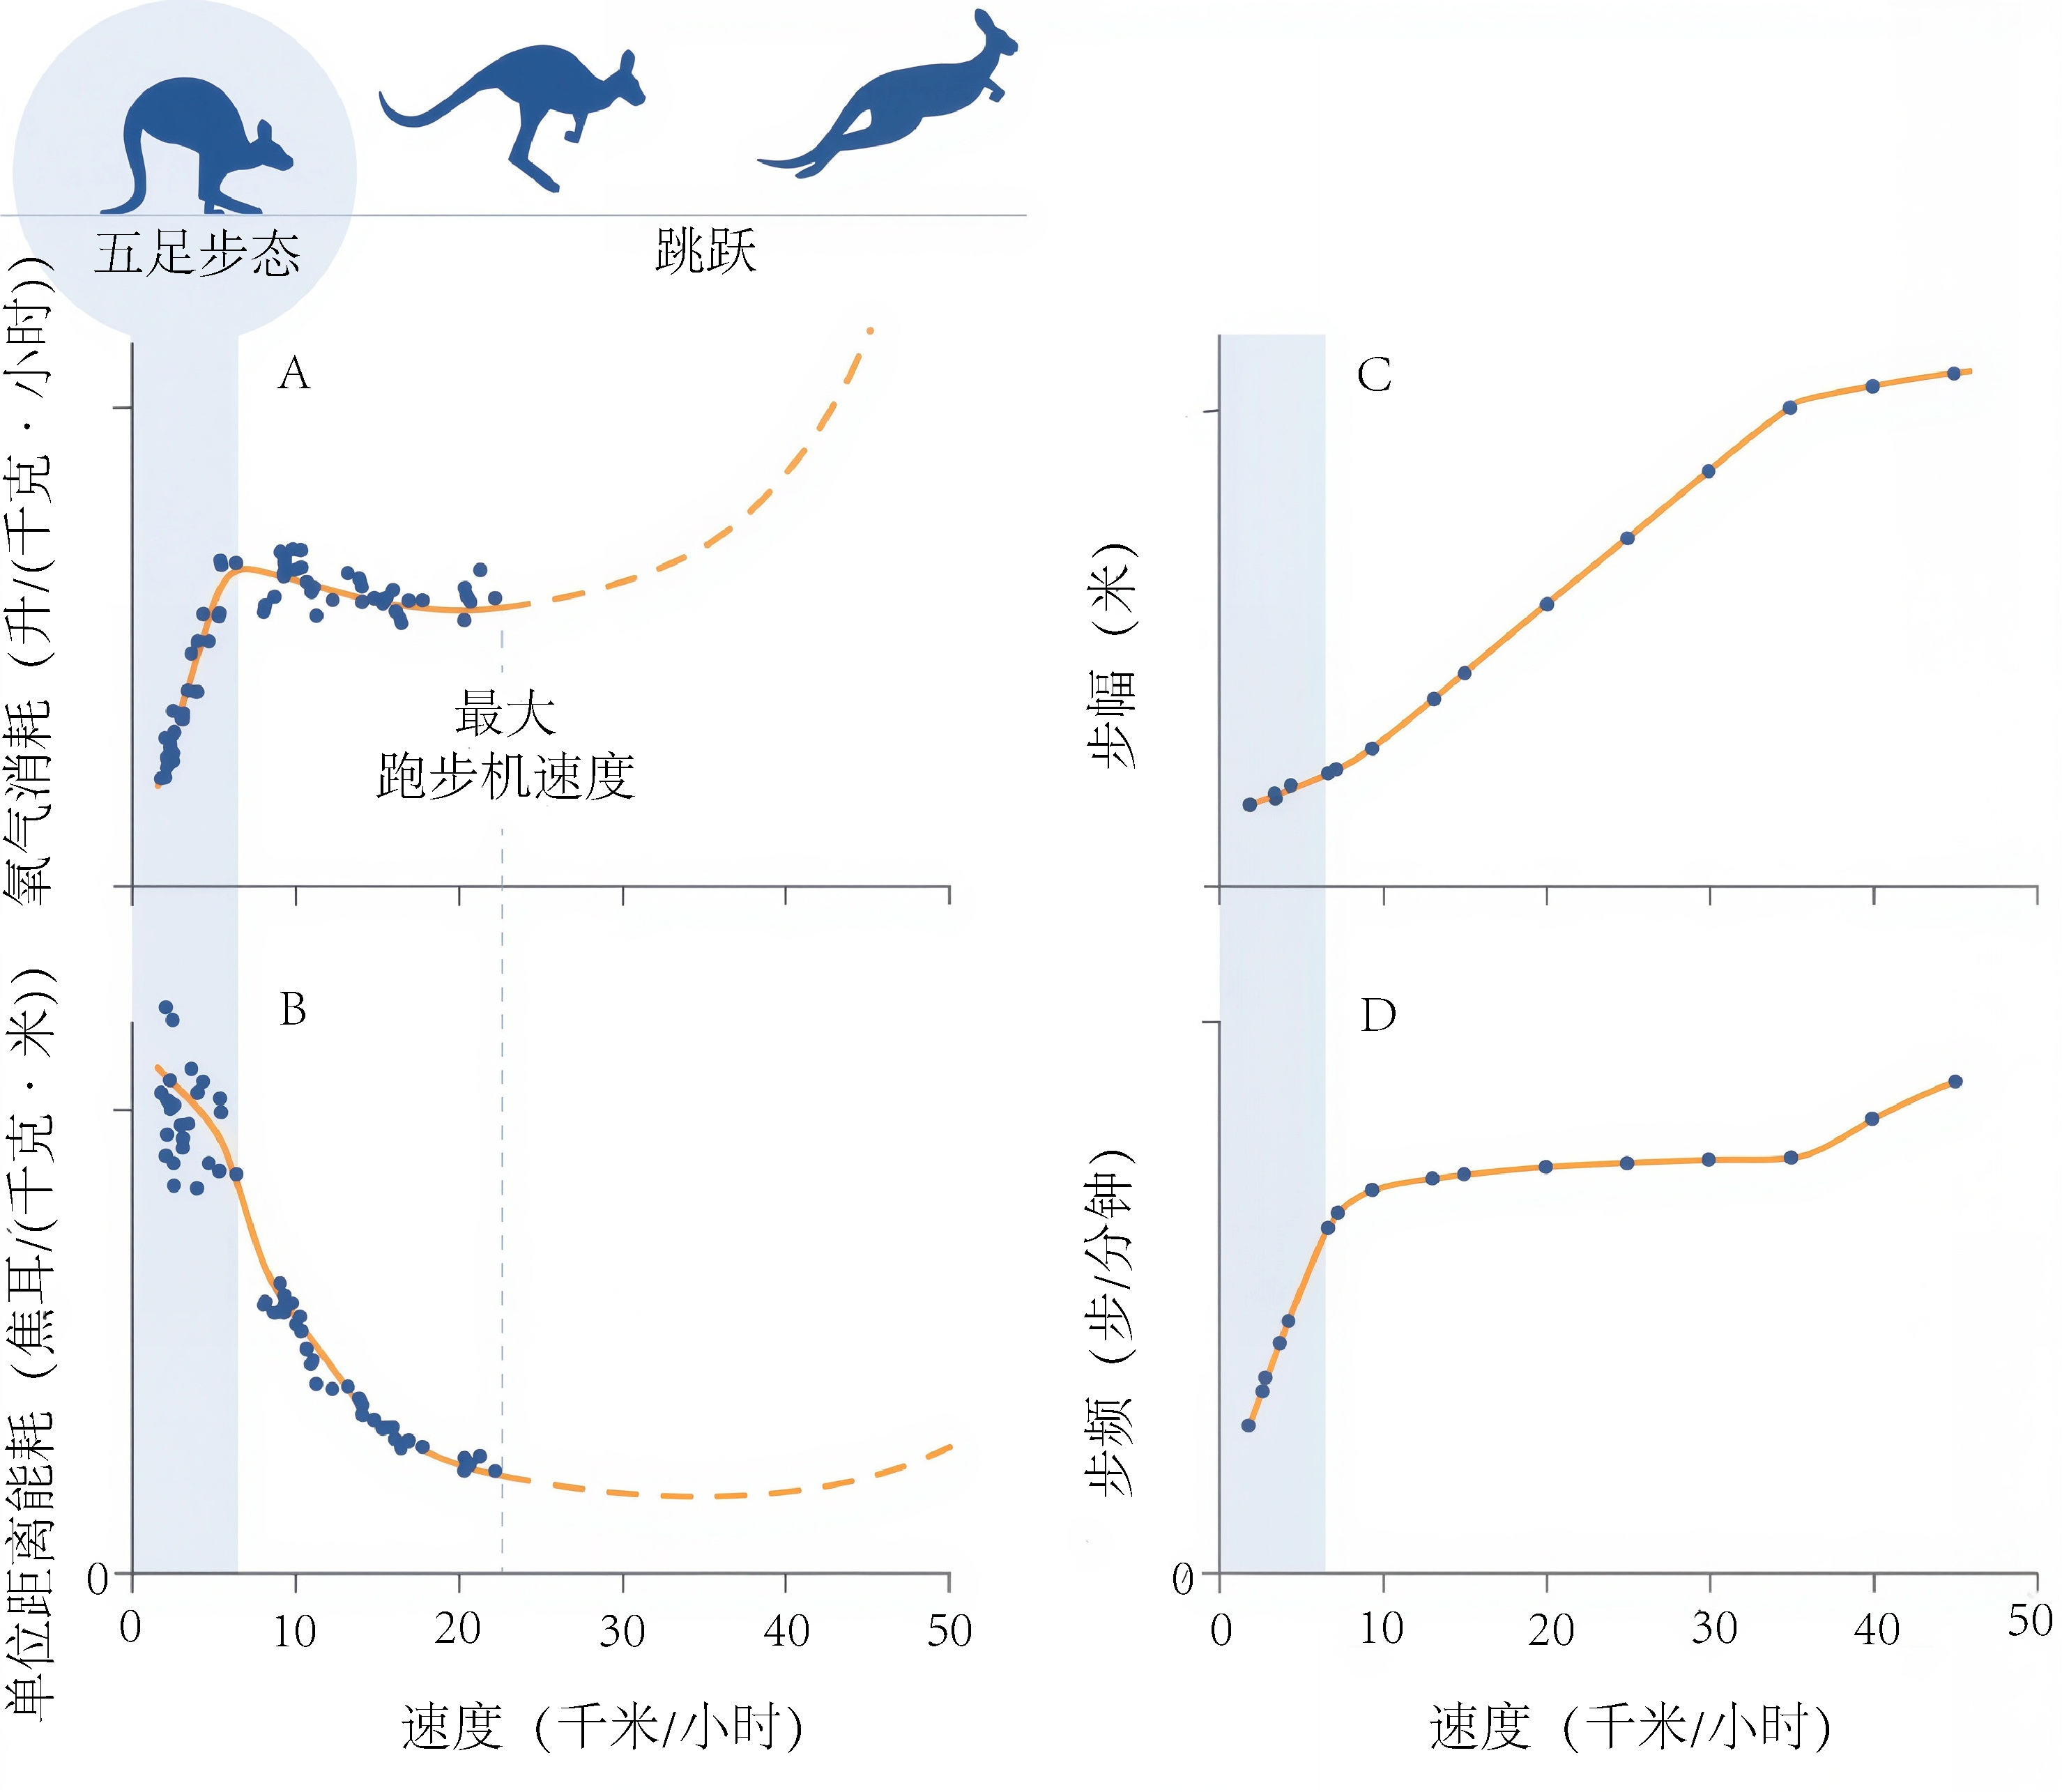
\includegraphics[width=1.0\linewidth]{chap3/3_7}
	\caption{袋鼠运动的能量学。
		在五足步态中,质量标准化的耗氧率随速度增加而增加。
		袋鼠在6-7公里/小时左右过渡到跳跃;
		随后耗氧量随速度增加而下降,直至20公里/小时左右达到最低值。
		Dawson\cite{dawson1977kangaroos}估算了无法在实验室研究的速度下的耗氧量(虚线)。
		在低速跳跃时,步频保持相对恒定,速度主要通过增加步幅来提高\cite{dawson1977kangaroos}。 \label{fig:3_7}}
\end{figure}


\section{跳跃机器人}

许多早期的步行机器人在运动过程中保持静态稳定,向前移动时重心保持在脚部上方。
20世纪80年代,马克$\cdot$雷伯特(Marc Raibert)和他的同事制造了第一批能够在高速运动中保持“动态平衡”的机器人,它们像跑步一样交替进行支撑和飞行。
这些早期的机器人跑步者只有一条腿,依靠运动来保持稳定,只能通过跳跃来保持直立。
这种巧妙的设计将控制问题集中在保持平衡上,同时避免了协调多条腿运动的复杂性。


Raibert 的第一个机器人用一条弹性腿在平面上跳跃(图~\ref{fig:3_8})。
该机器人受到机械约束以防止侧翻,并被拴在一台控制计算机和外部压缩空气及电源上。
腿部在可调节刚度的弹簧(气缸)上弹跳,弹簧为每次跳跃提供所需的能量。
控制器由三个独立组件组成:
第一个组件通过向气缸充气和放气来调节垂直运动,调整腿部刚度;
第二个组件通过在飞行过程中适当定位脚部来保持平衡;
第三个组件通过在站立时在腿和身体之间施加扭矩来稳定身体的姿态(倾斜度)。
腿部摆动是平衡和姿态控制器产生的臀部扭矩的自然结果。
例如,在飞行过程中,平衡控制器必须向前摆动腿部以准备下一个站立阶段。

\begin{figure}[!htb]
	\centering
	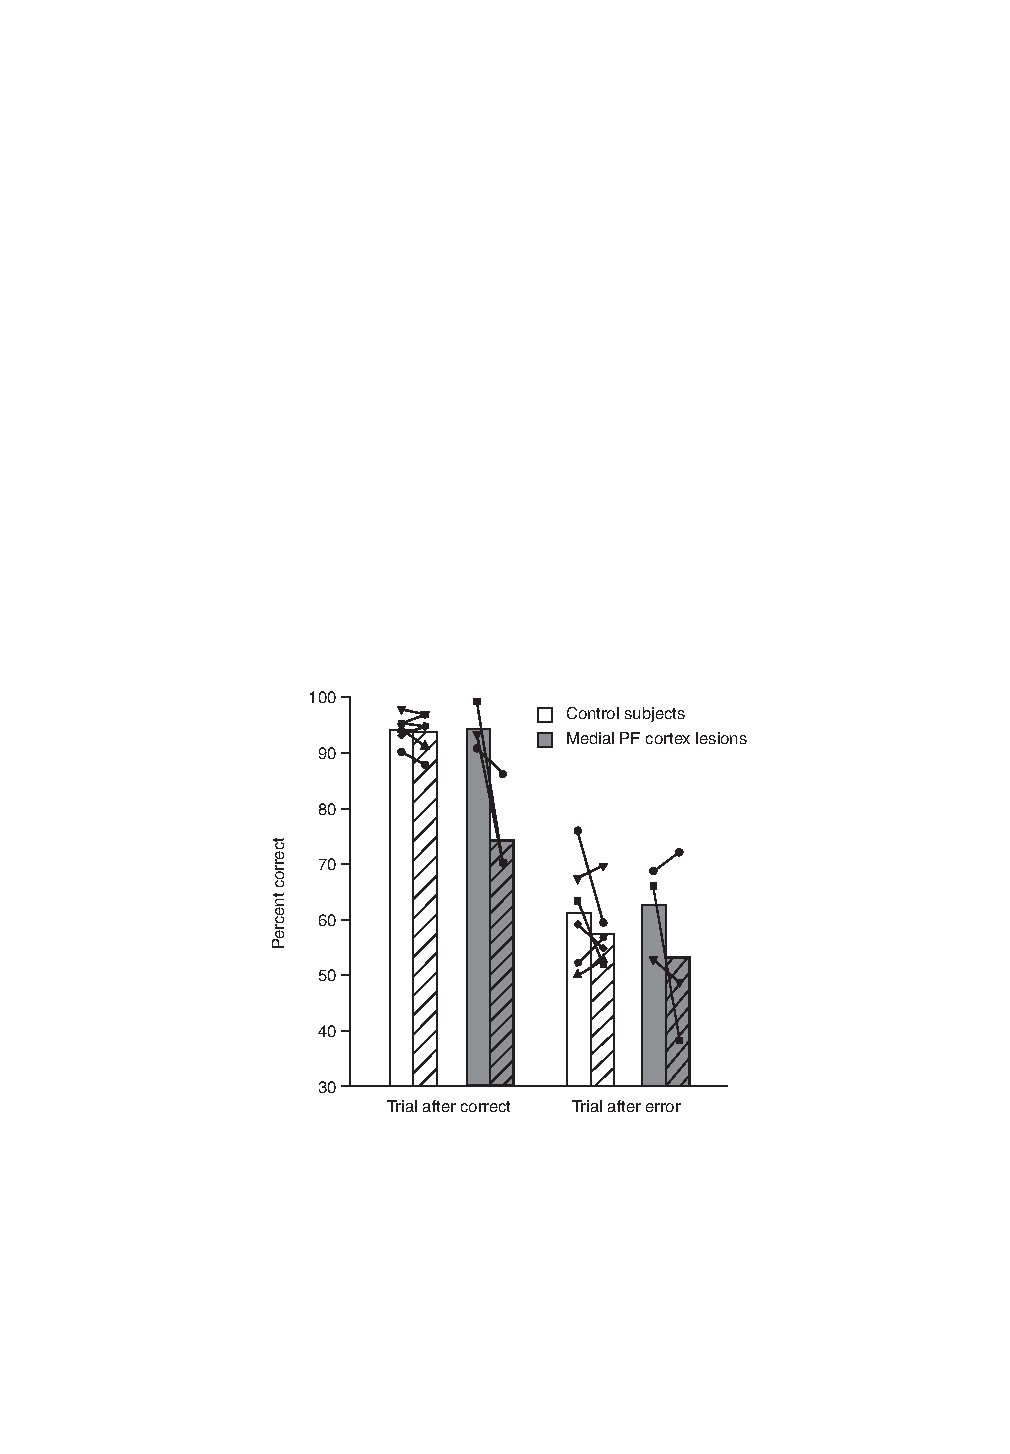
\includegraphics[width=1.0\linewidth]{chap3/3_8}
	\caption{Raibert 平面机器人的运动方式类似于跳跃的袋鼠,尽管它没有尾巴来控制俯仰。
		机载电子设备可以调节臀部角度和腿部刚度,以控制平衡、垂直运动和身体姿态。
		与有袋动物不同,该机器人只能在跳跃时保持平衡\cite{raibert1984machines}。 \label{fig:3_8}}
\end{figure}

同样的三段式控制策略也被用于动态平衡一个类似的3D跳跃机器人\cite{raibert1984machines}。
该机器人同样依靠一条弹性腿弹跳,每次跳跃时储存和释放能量。
然而,与其平面前身不同的是,机器人的躯干不受约束,因此平衡控制器可以调节其俯仰角和滚转角。
该机器人的最高速度可达2.2米/秒(慢跑速度),并且能够从外部扰动中恢复,这由机器人设计师自豪地提供。
Raibert后来于1992年创立了波士顿动力公司,该公司开发了一系列敏捷机器人。
这些机器人已经发展到两条腿和四条腿,但它们仍然基于相同的原理。
在近二十年开发尖端机器人之后,该公司宣布计划于2019年推出其首款商业模型——受犬类启发的SpotMini(图~\ref{fig:3_9})。


\begin{figure}[!htb]
	\centering
	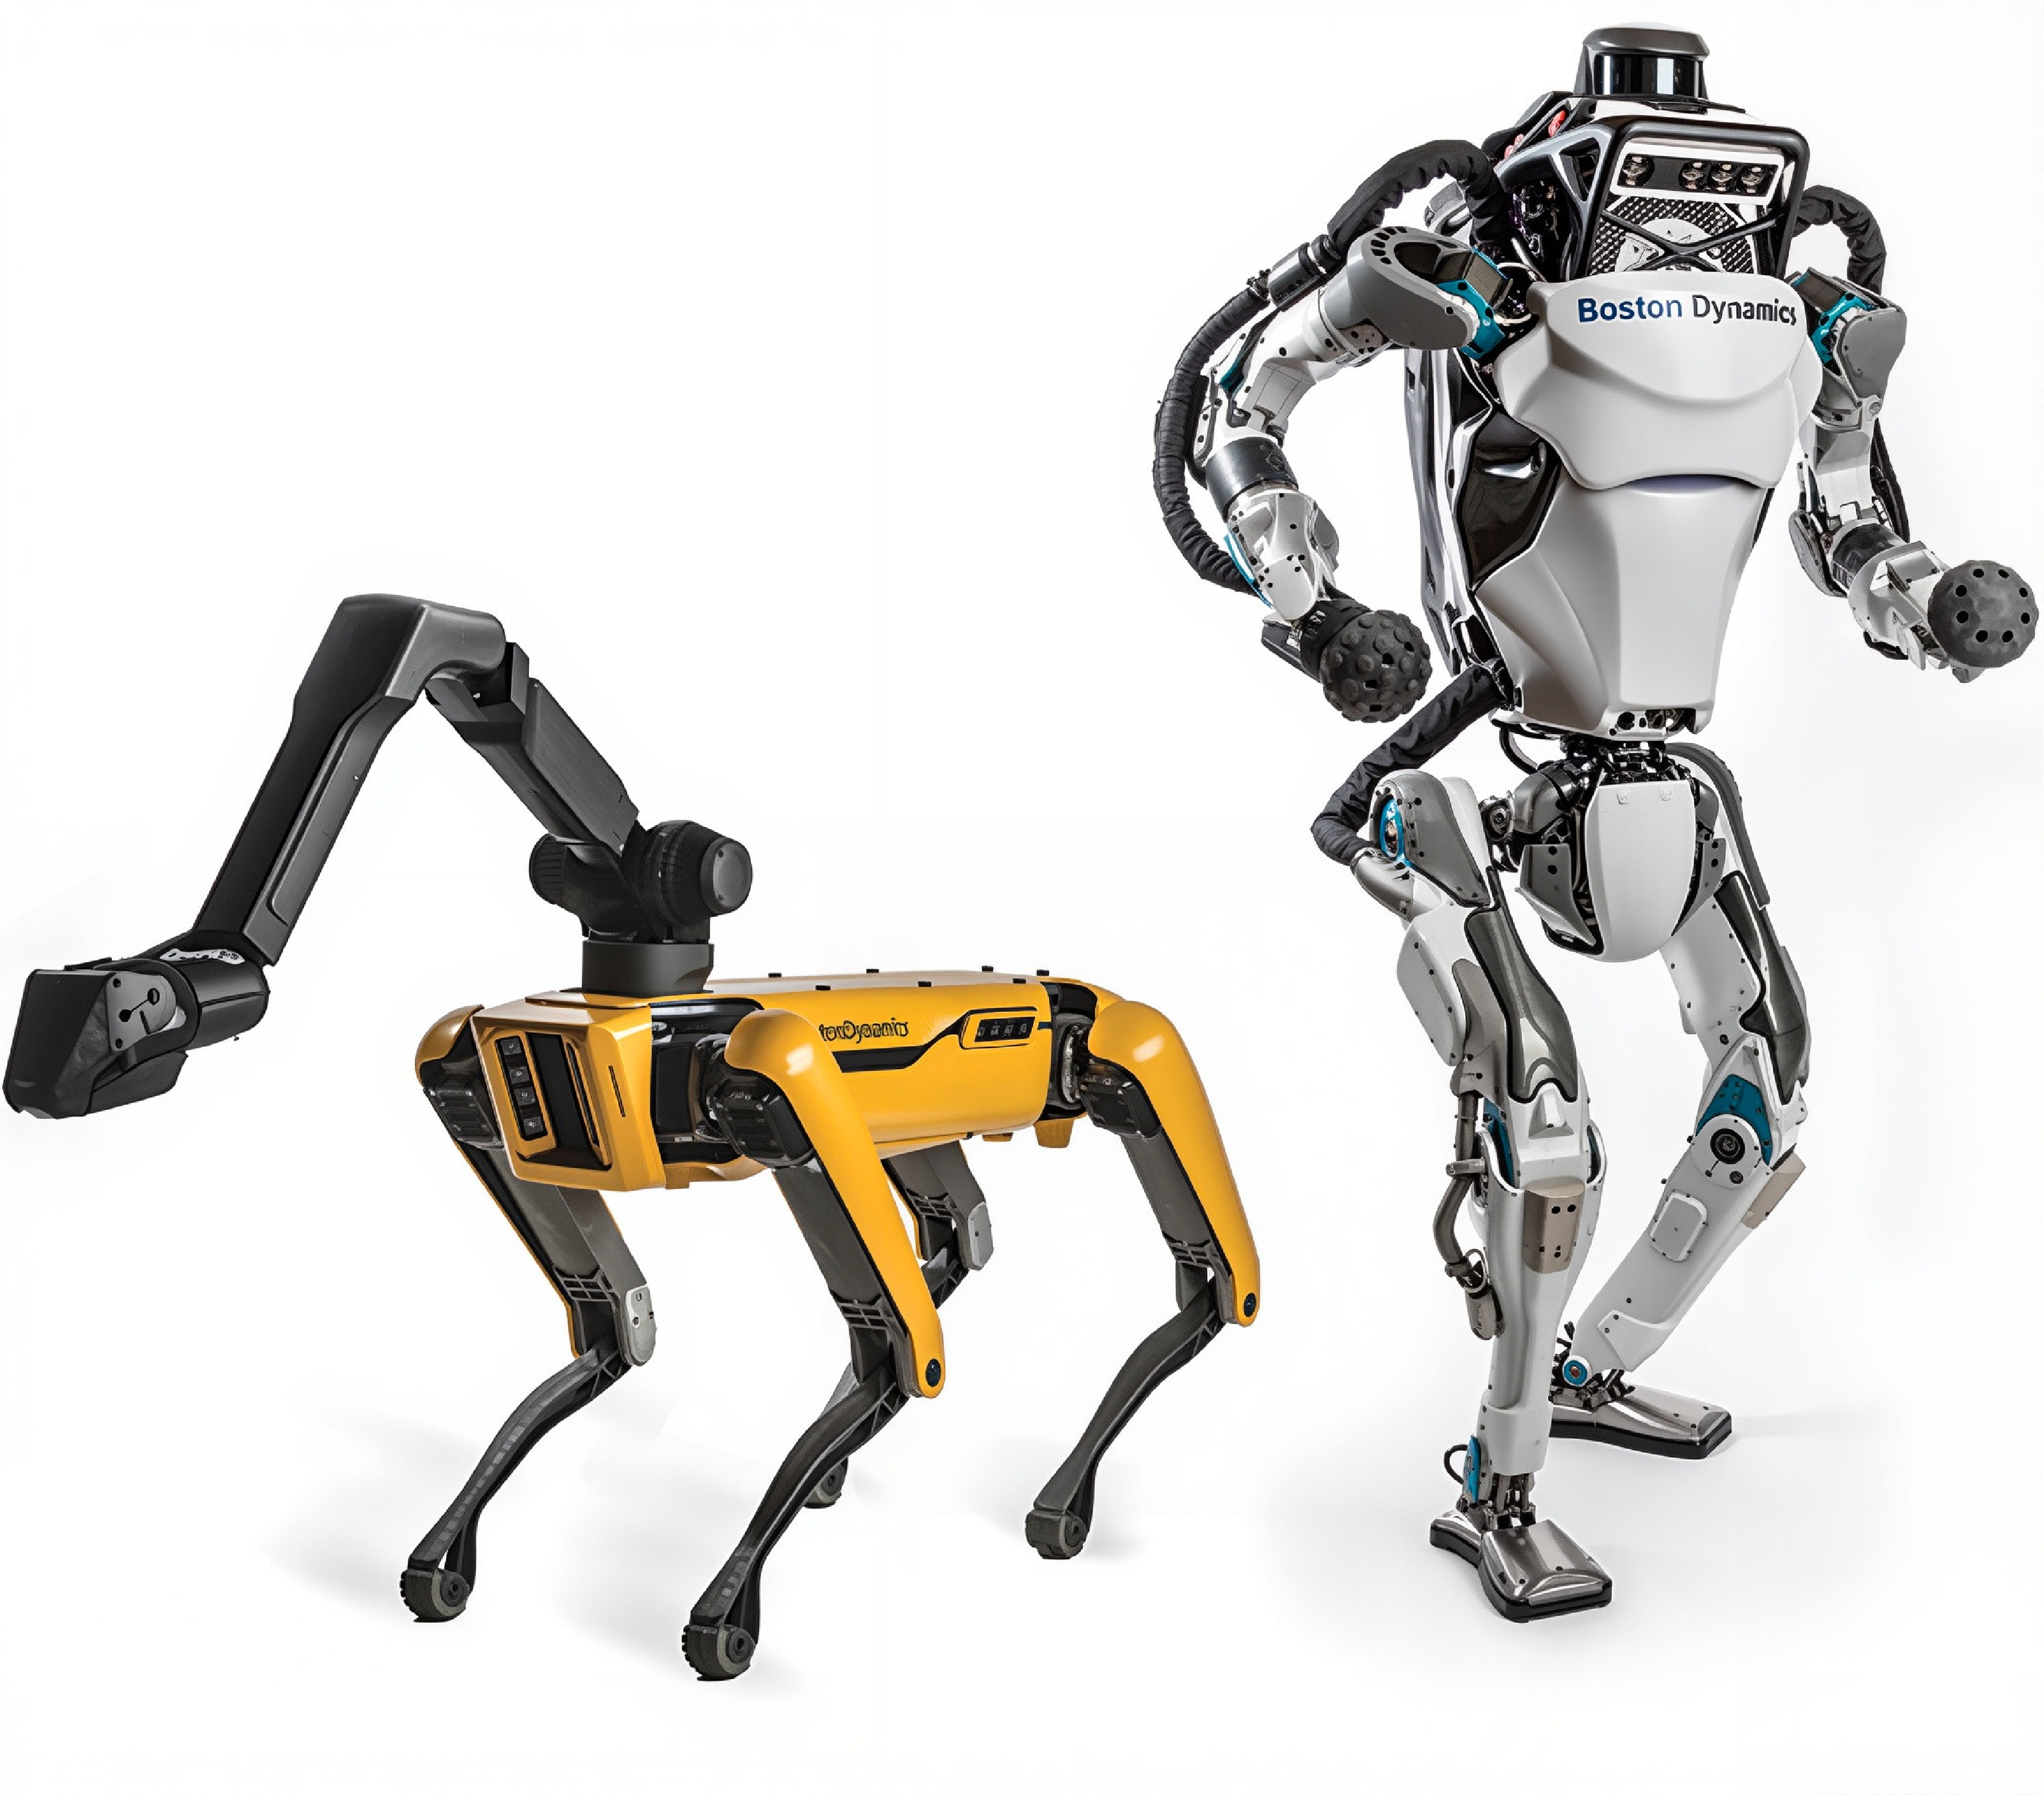
\includegraphics[width=1.0\linewidth]{chap3/3_9}
	\caption{现代跑步机器人的例子。
		Spot 机器人(左)和 Atlas 机器人(右)的照片由波士顿动力公司提供。 \label{fig:3_9}}
\end{figure}


\section{调谐轨迹}

20世纪70年代中期,托马斯$\cdot$麦克马洪接到了一个不寻常的求助电话。
哈佛大学正在修建一条新的室内跑道,承包商与田径教练在弯道坡度应该多大的问题上意见不合\cite{wingerson1983lion}。
在麦克马洪解决了这个问题(支持了田径教练的意见)后,他们又问了他另一个问题:跑道表面应该有多硬?


当时,传统观念认为跑道越硬越好,以尽量减少跑者双脚与地面的接触时间。
但麦克马洪质疑了这种观点。
在他看来,更柔顺(或“弹性”)的跑道可以通过增加步幅、步频或两者兼而有之来提高跑者的速度(回想一下公式~\ref{eq:3_1})。
他还提出理论,柔顺的跑道可以通过降低后脚掌着地的跑者所观察到的地面反作用力的初始峰值来降低受伤风险(图~\ref{eq:3_2})。


数学模型可以阐明这一理论。
麦克马洪与同事彼得$\cdot$格林一起,专注于跑步的站立阶段,这是步态周期中唯一一个跑道能够直接影响跑步者动态的阶段。
他们将跑步者建模为一个质量-弹簧-阻尼器系统,并与代表跑道的弹簧串联(图~\ref{fig:3_10})。
跑步者的弹簧反映了肌肉和肌腱的弹性特性;阻尼器反映了速度对肌肉力量的影响。
模型的最后一个组件是一个线性弹簧,它代表跑道的柔顺性,并寻求其最佳刚度。


\begin{figure}[!htb]
	\centering
	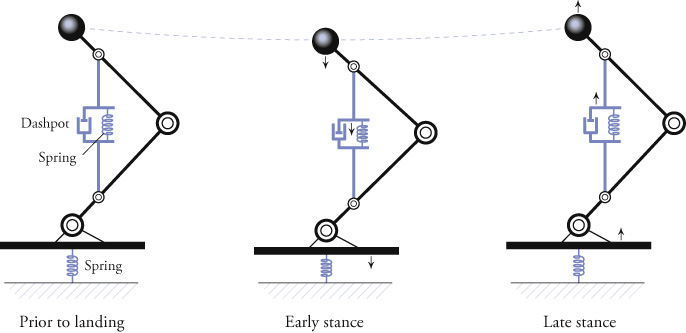
\includegraphics[width=1.0\linewidth]{chap3/3_10}
	\caption{McMahon 和 Greene 用于预测在柔顺跑道上跑步表现的概念模型。
		被动弹簧减震器系统代表肌肉的机械特性,脚下的弹簧代表跑道的柔顺性。
		分析了该系统在站立初期(中)的压缩和站立后期(右)的回弹动态,以找到最适合腿部特性的跑道弹簧刚度\cite{mcmahon1979influence}。 \label{fig:3_10}}
\end{figure}

该系统具有 2 个自由度,其动力学由两个二阶常微分方程控制,可从图~\ref{fig:3_11}~所示的示意图推导出来:

\begin{figure}[!htb]
	\centering
	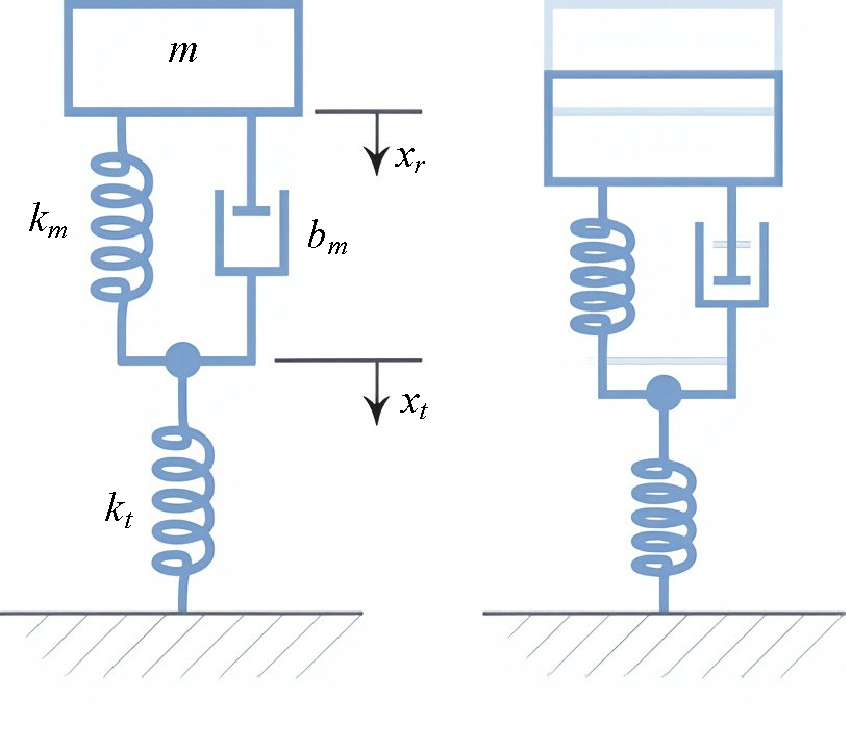
\includegraphics[width=1.0\linewidth]{chap3/3_11}
	\caption{用于推导图~\ref{fig:3_10}~所示概念模型运动方程的示意图。
		左图为系统处于平衡状态,右图为系统处于站立状态。
		跑步者的身体被建模为一个质量块 ($m$),其在弹簧(刚度为 $k_m$)和阻尼器(阻尼系数为 $b_m$)产生的力(代表腿部肌肉的综合作用)的作用下,发生位移 $x_r$ 的移动。
		脚下的小块跑道被建模为一个无质量物体,并通过一个代表跑道柔度的弹簧(刚度为 $k_t$)连接到地面\cite{mcmahon1979influence}。 \label{fig:3_11}}
\end{figure}

\begin{equation}
\begin{aligned}
	m \ddot{x}_t + 
	m_m ( \dot{x}_r - \dot{x}_t )
	k_m ( x_r - x_t ) = 0 \\
	b_m ( \dot{x}_r - \dot{x}_t )
	+ k_m ( x_r - x_t ) 
	- k_t x_t = 0
\end{aligned}
\end{equation}
% 
其中 $m$ 是跑步者身体的质量,$x_r$ 是其相对于平衡位置的位移,$x_t$ 是脚下跑道的位移,$b_m$ 是减震器的阻力,$k_m$ 和 $k_t$ 分别是肌肉和跑道弹簧的刚度。


McMahon 和 Greene 通过计算该系统的固有频率,并注意到足部在大约一次振动周期的一半后便会抬离地面,从而估算出了足部与地面的接触时间,该接触时间与履带刚度 $k_t$ 的关系。
他们的第一个意外发现是,在一系列中等刚度的履带上,接触时间比在非常坚硬的路面(例如混凝土路面)上跑步时的接触时间更短($t_0$;图 3.12)。
即使步幅保持不变,这一发现也令人预期跑步速度会有所提升,因为步频往往会随着接触时间的减少而增加。








